\documentclass[11pt,a4paper]{article}
\usepackage[T1]{fontenc}
\usepackage[margin=2.3cm]{geometry}
\usepackage{amsmath,amssymb}
\usepackage{graphicx}
\usepackage[dvipsnames]{xcolor}
\usepackage{enumitem}
\usepackage[colorlinks=true,linkcolor=blue,urlcolor=blue]{hyperref}
\setlength{\parskip}{0.6em}
\setlength{\parindent}{0pt}
\begin{document}

\begin{center}{\LARGE\bfseries opencrashsim}\\[0.4em]{\large Design a crumple zone with momentum and energy, in three sessions.}\\[0.2em]\small PAN IIT OSS explainer \textbullet{} secondary school to diploma / undergraduate (levels 3-5)\end{center}

\section*{Why this exists}
A car crash lasts less than a tenth of a second, but its physics is the physics of Newton's laws: momentum, impulse, work and energy. This explainer shows why stopping over a longer distance needs a smaller force and how a simple crumple-zone model can be simulated and checked against exact results.

\section*{The end goal}
Design crumple zones with momentum and energy balance. The end goal is to design a crumple zone on paper and in code using momentum and the energy balance: choose a plateau force and a crumple length that keep the deceleration within a target. The models are simplified and educational only, not a crashworthiness design tool.

\section*{How the three sessions build up}
\begin{enumerate}[nosep]
\item \textbf{Session 1: Why a car crumples: a longer stop means a smaller force} (Level 1, conceptual interactive model, 60 min).
\item \textbf{Session 2: Momentum, impulse and energy of a stop} (Level 2, mathematical engineering model, 75 min).
\item \textbf{Session 3: A crumple zone you can simulate and validate} (Level 3, simulation and validation, 90 min).
\end{enumerate}

\section{Session 1: Why a car crumples: a longer stop means a smaller force}

\subsection*{A. Real-world problem}
A car hits a wall. The wall does not move, so the car has to stop within whatever distance the car itself provides. A stiff, rigid front stops the car in a few centimetres and the force is enormous. A front that crumples stops it over about half a metre and the force is far smaller. How does the stopping distance control the force? (This is general physics education, not a vehicle safety guide.)

\subsection*{B. Concept and theory}
A car of mass m moving at speed v carries kinetic energy KE = (1/2) m v\textasciicircum{}2. To stop, all of that energy must be removed. A force F pushing back over a distance d does work F d. If the force is constant, setting work equal to energy gives F d = (1/2) m v\textasciicircum{}2, so F = m v\textasciicircum{}2 / (2 d). The force is inversely proportional to the distance: double the crumple distance and the force halves. Newton's second law F = m a turns the force into a deceleration a = v\textasciicircum{}2 / (2 d), which does not depend on the mass. We write a as a multiple of g = 9.81 m/s\textasciicircum{}2, so 'a = 20 g' means 20 times the pull of gravity. The speed must be in metres per second: divide km/h by 3.6.

\begin{itemize}[nosep]
\item m: mass of the car (kg)
\item v: speed just before the crash (m/s)
\item d: stopping distance (crumple distance) (m)
\item KE: kinetic energy (J)
\item F: average stopping force (N)
\item a: average deceleration (m/s\textasciicircum{}2)
\item g: gravitational acceleration, 9.81 (m/s\textasciicircum{}2)
\end{itemize}

\begin{equation*}
KE=\tfrac12 m v^2
\end{equation*}

\begin{equation*}
F\,d=\tfrac12 m v^2\quad\Longrightarrow\quad F=\dfrac{m v^2}{2d}
\end{equation*}

\begin{equation*}
a=\dfrac{F}{m}=\dfrac{v^2}{2d}\qquad\text{in g units: } \dfrac{a}{g}
\end{equation*}

\begin{center}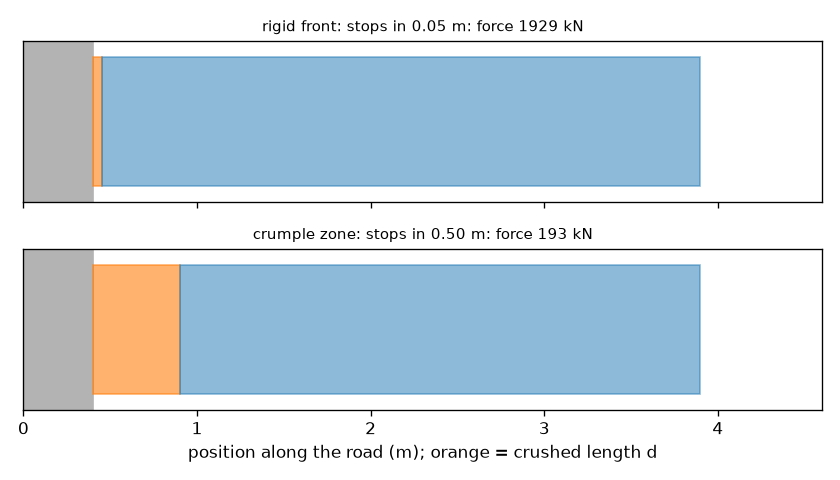
\includegraphics[width=0.85\linewidth]{figures/s01_car_wall.png}\\\small Rigid front (0.05 m of crush) versus crumple zone (0.50 m): about 1929 kN versus 193 kN.\end{center}

\subsection*{E. Worked example}
A 1000 kg car at 50 km/h is stopped by a crumple zone over 0.5 m. Find the average force and the deceleration in g.
\begin{enumerate}[nosep]
\item Convert the speed: 50 km/h / 3.6 = 13.89 m/s.
\item Kinetic energy: KE = 0.5 * 1000 * 13.89\textasciicircum{}2 = 96450 J (96.5 kJ).
\item Force: F = KE / d = 96450 / 0.5 = 192900 N = 192.9 kN.
\item Deceleration: a = F / m = 192900 / 1000 = 192.9 m/s\textasciicircum{}2.
\item In g: 192.9 / 9.81 = 19.7 g.
\item Sanity check: a = v\textasciicircum{}2 / (2 d) = 192.9 / 1.0 = 192.9 m/s\textasciicircum{}2, the same.
\end{enumerate}
\textbf{Answer.} The average force is 192.9 kN, a deceleration of 19.7 g.

\subsection*{F. Questions}
\begin{enumerate}[nosep]
\item \textbf{Conceptual.} A heavy truck and a small car hit a wall at the same speed and both stop in 0.5 m. Which has the larger average force? Which has the larger deceleration? Explain.
\item \textbf{Numerical.} A 1500 kg car at 36 km/h is stopped in 0.4 m. Find the average force (in kN) and the deceleration (in g). Check your answer another way.
\item \textbf{Graph and simulation interpretation.} On the force-versus-distance graph for a 1000 kg car at 50 km/h the force at d = 0.2 m is about 482 kN. Without a calculator, what is the force at d = 0.4 m and at d = 0.1 m? What is the curve called and why is it never zero?
\item \textbf{Design and optimisation challenge.} Design: a 1000 kg car at 50 km/h must be stopped with an average force of at most 150 kN. What is the smallest crumple distance? Pick a practical value to the nearest 0.05 m and state the trade-off.
\end{enumerate}

\section{Session 2: Momentum, impulse and energy of a stop}

\subsection*{A. Real-world problem}
A crash lasts only a few hundredths of a second. Session 1 used energy and distance. There is a second, independent way: momentum and time. Can the two views agree? And can we use them to answer a design question: how much crumple distance keeps the driver's deceleration below 20 g (a commonly quoted rough scale for brief loads, not a safety rule) when the car hits at 50 km/h? What changes at 100 km/h? This lesson is general physics education and makes no injury predictions.

\subsection*{B. Concept and theory}
Momentum is p = m v. Newton's second law says F = dp/dt, so a force F acting for a short time dt delivers an impulse F dt equal to the change in momentum. For a constant force lasting a time t that stops the car, F t = m v. For the same stop, the work-energy theorem gives F d = (1/2) m v\textasciicircum{}2. With constant deceleration the average speed during the stop is v/2, so d = (v/2) t and t = 2 d / v. Putting this t into F t = m v returns F = m v\textasciicircum{}2 / (2 d): the two views agree. The deceleration is a = F / m = v\textasciicircum{}2 / (2 d) and the g-force is a / g. Solving for the distance needed to stay below a g-limit: d = v\textasciicircum{}2 / (2 (limit) g). Because d is proportional to v\textasciicircum{}2, doubling the speed needs four times the distance for the same g.

\begin{itemize}[nosep]
\item p: momentum m v (kg m/s)
\item F t: impulse of a constant force (N s)
\item t: duration of the stop (s)
\item d: crumple (stopping) distance (m)
\item a: average deceleration (m/s\textasciicircum{}2)
\item g-limit: chosen limit on a / g (20 here) (no unit)
\item v: impact speed (m/s)
\end{itemize}

\begin{equation*}
F\,t=m v\qquad F\,d=\tfrac12 m v^2
\end{equation*}

\begin{equation*}
t=\dfrac{2d}{v}\quad\Longrightarrow\quad F=\dfrac{m v}{t}=\dfrac{m v^2}{2d}
\end{equation*}

\begin{equation*}
a=\dfrac{v^2}{2d},\qquad \text{g-force}=\dfrac{a}{g}
\end{equation*}

\begin{equation*}
d_{\min}=\dfrac{v^2}{2\,(\text{limit})\,g}\qquad v_{\max}=\sqrt{2\,(\text{limit})\,g\,d}
\end{equation*}

\begin{center}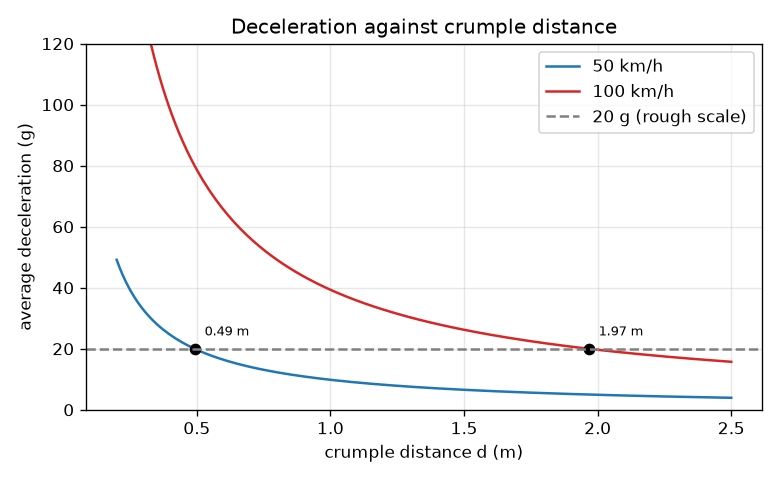
\includegraphics[width=0.85\linewidth]{figures/s02_decel_vs_distance.png}\\\small Deceleration against crumple distance at 50 and 100 km/h; the 20 g line is crossed at 0.49 m and 1.97 m.\end{center}

\subsection*{E. Worked example}
Find the crumple distance that keeps a 1000 kg car at 50 km/h to 20 g, the duration of the stop, and the force. Then do the same at 100 km/h.
\begin{enumerate}[nosep]
\item v = 50 / 3.6 = 13.89 m/s. The limit is a = 20 g = 20 * 9.81 = 196.2 m/s\textasciicircum{}2.
\item Distance: d = v\textasciicircum{}2 / (2 a) = 192.9 / (2 * 196.2) = 0.4917 m.
\item Time: t = 2 d / v = 2 * 0.4917 / 13.89 = 0.0708 s = 70.8 ms.
\item Force by impulse: F = m v / t = 1000 * 13.89 / 0.0708 = 196 kN. By energy: F = KE / d = 96450 / 0.4917 = 196 kN. They agree.
\item At 100 km/h: v = 27.78 m/s, so d = 771.6 / 392.4 = 1.966 m and t = 141.6 ms. The speed doubled, so the distance is 4 times as large (4 * 0.4917 = 1.967 m).
\end{enumerate}
\textbf{Answer.} About 0.49 m at 50 km/h (70.8 ms, 196 kN) and about 1.97 m at 100 km/h (141.6 ms): the same g needs 4 times the distance.

\subsection*{F. Questions}
\begin{enumerate}[nosep]
\item \textbf{Conceptual.} Why does doubling the speed need four times the crumple distance for the same deceleration, rather than twice?
\item \textbf{Numerical.} A 1000 kg car hits at 80 km/h. What crumple distance keeps the average deceleration at or below 20 g? What speed can a 0.6 m crumple zone handle at 20 g?
\item \textbf{Graph and simulation interpretation.} On the graph, a 1 m crumple distance at 50 km/h and at 100 km/h gives what g-forces? Which stays below the 20 g line?
\item \textbf{Design and optimisation challenge.} Design: a car must meet 20 g at 64 km/h but the crumple zone is limited to 0.6 m. Is that possible? If not, what is the least distance, and what are the options (lower speed, higher g, more distance)? State the trade-offs.
\end{enumerate}

\section{Session 3: A crumple zone you can simulate and validate}

\subsection*{A. Real-world problem}
Real crumple zones do not push back with one constant force. The front first resists more and more, then collapses at a roughly steady force (the plateau), and if it is used up the stiff passenger cell is next and the force jumps. Can we model this with a few lines of code, step it through time, check it against the exact formulas from Sessions 1 and 2, and use it to choose a plateau force and a crumple length for a small car at 56 km/h? This is a classroom model: not a crashworthiness design tool, and it makes no injury predictions.

\subsection*{B. Concept and theory}
The car is one lump of mass m crushing a front structure that resists with a force F(x) that depends on the crush distance x. The curve has three parts: a short ramp from 0 to the plateau force Fp over a length XR = 0.05 m, a constant plateau Fp up to the crumple length Lc, and beyond Lc a very stiff passenger cell with F = Fp + k (x - Lc), k = 3e7 N/m. Newton's law is m dv/dt = -(F(x) + c v) and dx/dt = v, with an optional damping coefficient c (default 0). We step these in time with the fourth-order Runge-Kutta method (RK4) and shorten the last step so the car stops exactly at v = 0. The work done by the force is the area under F(x), and the energy balance reads KE0 = work in the crumple zone and cell + energy lost in the damper + residual KE. If the crash ends on the plateau the exact answers are d = KE0 / Fp + XR / 2 and peak deceleration Fp / m. For two cars m1 and m2 meeting head on, momentum is conserved; if they lock together (perfectly inelastic) vf = (m1 v1 + m2 v2) / (m1 + m2) and the energy to be crushed is (1/2) mu v\_rel\textasciicircum{}2 with mu = m1 m2 / (m1 + m2). The same simulation runs with mass mu at the relative speed, through both crumple zones in series.

\begin{itemize}[nosep]
\item m: car mass (kg)
\item x: crush distance (m)
\item Fp: plateau force (N)
\item Lc: crumple length (m)
\item XR: length of the force ramp (0.05) (m)
\item k: stiffness of the passenger cell (3e7) (N/m)
\item c: damping coefficient (default 0) (N s/m)
\item mu: reduced mass of two cars (kg)
\item v\_rel: relative speed of two cars (m/s)
\end{itemize}

\begin{equation*}
F(x)=\begin{cases}F_p\,x/X_R & 0\le x<X_R\\ F_p & X_R\le x\le L_c\\ F_p+k\,(x-L_c) & x>L_c\end{cases}
\end{equation*}

\begin{equation*}
m\,\dfrac{dv}{dt}=-\big(F(x)+c\,v\big),\qquad \dfrac{dx}{dt}=v
\end{equation*}

\begin{equation*}
d=\dfrac{KE_0}{F_p}+\dfrac{X_R}{2},\qquad a_{\max}=\dfrac{F_p}{m}
\end{equation*}

\begin{equation*}
KE_0=\int_0^{x_{\rm end}}F\,dx+\int c\,v^2\,dt+KE_{\rm end}
\end{equation*}

\begin{equation*}
v_f=\dfrac{m_1 v_1+m_2 v_2}{m_1+m_2},\qquad \Delta KE=\tfrac12\,\mu\,v_{\rm rel}^2,\quad \mu=\dfrac{m_1 m_2}{m_1+m_2}
\end{equation*}

\begin{center}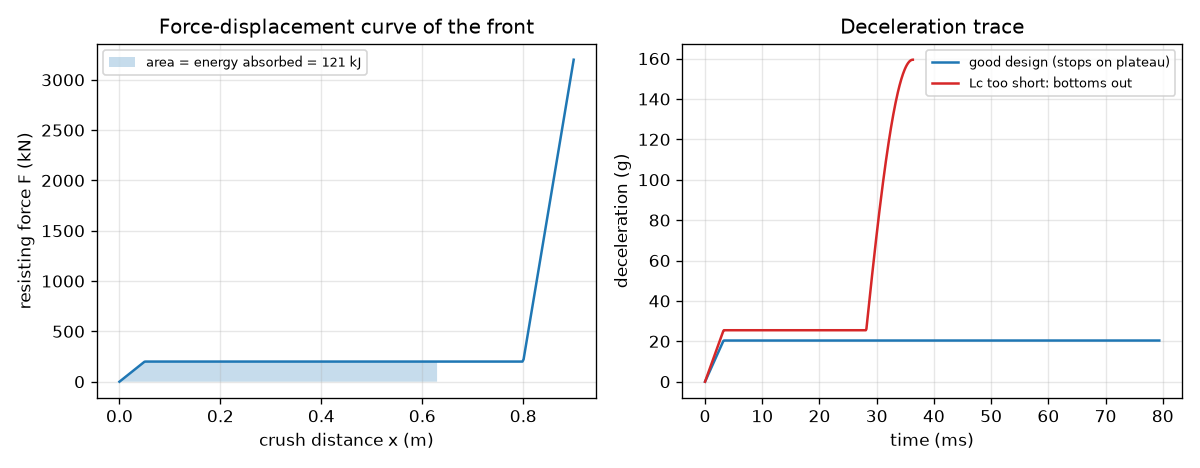
\includegraphics[width=0.85\linewidth]{figures/s03_force_and_trace.png}\\\small Force-displacement curve (left) and deceleration traces of a good design and a design that bottoms out (right).\end{center}

\subsection*{E. Worked example}
A 1000 kg car hits a rigid barrier at 56 km/h with Fp = 200 kN and Lc = 0.8 m. Find the stopping distance and the peak deceleration, and check them against the simulation and the energy balance.
\begin{enumerate}[nosep]
\item v = 56 / 3.6 = 15.556 m/s, so KE0 = 0.5 * 1000 * 15.556\textasciicircum{}2 = 120988 J (121.0 kJ).
\item The ramp (0 to 0.05 m) absorbs half of Fp * XR = 0.5 * 200000 * 0.05 = 5000 J.
\item The remaining 120988 - 5000 = 115988 J is absorbed on the plateau: 115988 / 200000 = 0.5799 m.
\item Total stopping distance d = 0.05 + 0.5799 = 0.6299 m. It is less than Lc = 0.8 m, so the crash ends on the plateau and the formula applies (equivalently KE0 / Fp + XR / 2 = 0.6049 + 0.025).
\item Peak deceleration = Fp / m = 200000 / 1000 = 200 m/s\textasciicircum{}2 = 20.39 g.
\item The RK4 simulation gives 0.6299 m, 20.39 g and a stop time of 79.4 ms, matching the exact values; the energy balance KE0 = crumple work + residual KE closes to about 1e-11 of KE0.
\end{enumerate}
\textbf{Answer.} Stopping distance 0.630 m, peak deceleration 20.4 g, stop time 79.4 ms; the simulation matches and the energy balance closes.

\subsection*{F. Questions}
\begin{enumerate}[nosep]
\item \textbf{Conceptual.} For a fixed crumple length and impact energy, why is a flat force plateau the best force-displacement curve for keeping the peak deceleration low?
\item \textbf{Numerical.} A 1200 kg car hits a barrier at 40 km/h; its crumple zone has Fp = 150 kN, XR = 0.05 m and a long length. Find the stopping distance and the peak deceleration.
\item \textbf{Graph and simulation interpretation.} In the deceleration-trace figure the failing design is flat at 25.5 g for about 28 ms and then climbs to 159 g. What happened, which part of the force curve produced the spike, and why does it come at the end of the crash?
\item \textbf{Design and optimisation challenge.} Design: for a 1000 kg car at 56 km/h choose Fp (steps of 10 kN) and Lc (steps of 0.05 m) so that peak deceleration is at most 22 g, Lc is at most 0.65 m and the car stops within 95 percent of Lc. Justify your choice.
\end{enumerate}

\section{Real-world mini-project}
\textbf{Choose the crumple zone for a small car at 56 km/h.} A small car of 1000 kg hits a rigid barrier at 56 km/h. Using \texttt{simulate\_crash} from Session 3, choose the plateau force Fp (steps of 10 kN, from 100 to 400 kN) and the crumple length Lc (steps of 0.05 m, from 0.30 to 0.70 m) so that three limits hold: peak deceleration at most 25 g (a teaching target, not a safety rule), a crumple length of at most 0.70 m (the space under the bonnet), and the car stops within 95 percent of Lc (a safety margin so the zone does not bottom out). Among the designs that pass, pick the one with the lowest peak deceleration, and explain what you gave up for it. This is a classroom exercise in a simplified model, not a real vehicle design.

\section{The path ahead}
\begin{enumerate}[nosep]
\item \textbf{Session 4: Add an occupant and a belt.} A second mass of 75 kg connected to the car by a belt with 30 mm slack, 80 kN/m stiffness and 1500 N s/m damping, with the belt reaction acting back on the car.
\item \textbf{Session 5: A staged crumple profile.} A force law with two plateaus and a transition length, swept over 40, 56 and 64 km/h.
\item \textbf{Session 6: Rebound and restitution.} An unloading path for the force curve so that the car can leave the barrier.
\item \textbf{Session 7: Off-centre crash with yaw.} A 2D rigid car with yaw inertia 1500 kg m\textasciicircum{}2 hitting a barrier 0.5 m off the centreline with the same plateau force law.
\item \textbf{Session 8: Reproduce the Target animation.} A side-by-side GIF of a bottoming-out design and a tuned design, each with a car picture, a live deceleration trace and an energy split.
\end{enumerate}

\section{Answers and hints}

\subsection*{Session 1}
\begin{enumerate}[nosep]
\item \textbf{Conceptual.} Hint: Compare F = m v\textasciicircum{}2 / (2 d) and a = v\textasciicircum{}2 / (2 d). Solution: The truck has the larger force because F is proportional to m. The deceleration a = v\textasciicircum{}2 / (2 d) has no mass in it, so both have the same deceleration. The truck's occupants feel the same g, but the truck's structure must carry a bigger force, which is why heavy vehicles need stronger, longer structures.
\item \textbf{Numerical.} Hint: 36 km/h is 10 m/s. Use F = m v\textasciicircum{}2 / (2 d) and a = F / m. Solution: v = 36 / 3.6 = 10 m/s. F = 1500 * 10\textasciicircum{}2 / (2 * 0.4) = 150000 / 0.8 = 187500 N = 187.5 kN. a = 187500 / 1500 = 125 m/s\textasciicircum{}2 = 125 / 9.81 = 12.7 g. Check: a = v\textasciicircum{}2 / (2 d) = 100 / 0.8 = 125 m/s\textasciicircum{}2, the same.
\item \textbf{Graph and simulation interpretation.} Hint: F is proportional to 1 / d. Solution: Doubling the distance halves the force: 241 kN at 0.4 m. Halving the distance doubles it: 965 kN at 0.1 m. The curve is a hyperbola F = KE / d. It never reaches zero because a finite energy needs some force over any finite distance; it gets small only for very long stops.
\item \textbf{Design and optimisation challenge.} Hint: Rearrange F = KE / d to d = KE / F and round up. Solution: KE = 96450 J, so d = 96450 / 150000 = 0.643 m. Round up to 0.65 m (rounding down would exceed 150 kN): F = 96450 / 0.65 = 148.4 kN, a = 14.8 g. Trade-off: a longer crumple zone lowers the force but makes the car longer or heavier, and the model assumes a constant force, which a real structure only approximates.
\end{enumerate}

\subsection*{Session 2}
\begin{enumerate}[nosep]
\item \textbf{Conceptual.} Hint: Look at where v appears in d = v\textasciicircum{}2 / (2 a). Solution: The distance needed is d = v\textasciicircum{}2 / (2 a), and v appears squared. Equivalently the kinetic energy grows as v\textasciicircum{}2, and at a fixed force the distance to absorb it must grow as v\textasciicircum{}2. Doubling v makes v\textasciicircum{}2 four times larger. In the time view the stop also lasts twice as long, and the average speed during it is twice as large, so distance = average speed times time is four times larger.
\item \textbf{Numerical.} Hint: 80 km/h is 22.22 m/s. Use d = v\textasciicircum{}2 / (2 * 20 * 9.81) and v = sqrt(2 * 20 * 9.81 * d). Solution: d = 22.22\textasciicircum{}2 / (2 * 20 * 9.81) = 493.8 / 392.4 = 1.26 m. For d = 0.6 m: v = sqrt(392.4 * 0.6) = sqrt(235.4) = 15.34 m/s = 55.2 km/h. Check: a = 15.34\textasciicircum{}2 / (2 * 0.6) = 196.2 m/s\textasciicircum{}2 = 20 g.
\item \textbf{Graph and simulation interpretation.} Hint: Read the two curves at d = 1.0 m, or compute a = v\textasciicircum{}2 / (2 d). Solution: At 50 km/h: a = 192.9 / 2 = 96.4 m/s\textasciicircum{}2 = 9.8 g, below the 20 g line. At 100 km/h: a = 771.6 / 2 = 385.8 m/s\textasciicircum{}2 = 39.3 g, above it, four times the 50 km/h value. The red curve only drops below the 20 g line beyond d = 1.97 m.
\item \textbf{Design and optimisation challenge.} Hint: Compute d for 64 km/h = 17.78 m/s and compare with 0.6 m. Solution: d = 17.78\textasciicircum{}2 / 392.4 = 316.0 / 392.4 = 0.805 m, which is more than 0.6 m, so it is not possible: with 0.6 m the deceleration would be 316 / 1.2 / 9.81 = 26.8 g. Options: lengthen the crumple zone to 0.81 m (longer, heavier car), accept a higher g (a different, harder target) or reduce the speed the zone is designed for (0.6 m handles 55.2 km/h at 20 g). Any real design balances these with cost, space, pedestrian safety and many other things the model ignores.
\end{enumerate}

\subsection*{Session 3}
\begin{enumerate}[nosep]
\item \textbf{Conceptual.} Hint: The area under the curve must equal the kinetic energy. Solution: The area under F(x) over the crush length equals the energy to absorb, so the average force is fixed at KE0 / d. Any curve that is higher than the average somewhere must be lower elsewhere, and its peak is above the average. A flat curve has no peak above the average, so for the same energy and length it gives the lowest possible peak deceleration. Real structures cannot be perfectly flat and need a ramp at the start, which is why the model has one.
\item \textbf{Numerical.} Hint: v = 11.11 m/s. Use d = KE0 / Fp + XR / 2 and a = Fp / m. Solution: KE0 = 0.5 * 1200 * 11.11\textasciicircum{}2 = 74074 J. d = 74074 / 150000 + 0.025 = 0.4938 + 0.025 = 0.519 m. Peak a = 150000 / 1200 = 125 m/s\textasciicircum{}2 = 12.7 g. Check that Lc is at least 0.52 m, otherwise the zone bottoms out.
\item \textbf{Graph and simulation interpretation.} Hint: Where is the car when the force curve passes x = Lc? Solution: The crumple length Lc = 0.35 m was used up while the car still had kinetic energy (the plateau only absorbed about 81 kJ of the 121 kJ). The car then compressed the stiff passenger cell, where the force rises steeply with x. Since the car's speed is lowest at the end, the spike occurs at the end of the crash, just before the car stops, and it is far larger than the plateau value because the cell is nearly rigid. This is the bottoming-out failure.
\item \textbf{Design and optimisation challenge.} Hint: Peak deceleration is Fp / (m g), and the stop distance is KE0 / Fp + XR / 2 = 120988 / Fp + 0.025. Solution: The peak limit gives Fp \textless{}= 22 * 1000 * 9.81 = 215.8 kN. The margin gives 120988 / Fp + 0.025 \textless{}= 0.95 * 0.65 = 0.6175 m, so Fp \textgreater{}= 204.2 kN. On a 10 kN grid only Fp = 210 kN works, with Lc = 0.65 m: peak 21.4 g and stop distance 0.601 m. Fp = 200 kN stops in 0.630 m (too long) and Fp = 220 kN gives 22.4 g (too high). The window is narrow: a tighter g limit needs a longer crumple zone.
\end{enumerate}

\section{How to join}
Read \texttt{CONTRIBUTING.md} in the repository, then pick an issue labelled \texttt{good first issue}. Repository: \url{https://github.com/KrunalPanchal1995/opencrashsim}

\end{document}
